\documentclass[a4paper,9pt]{beamer}
%
% Choose how your presentation looks.
%
% For more themes, color themes and font themes, see:
% http://deic.uab.es/~iblanes/beamer_gallery/index_by_theme.html
%
 \mode<presentation>
{
  \usetheme{Singapore}      % or try Darmstadt, Madrid, Warsaw, ...
  \usecolortheme{} % or try albatross, beaver, crane, ...
  %\usefonttheme{serif}  % or try serif, structurebold, ...
  \mode<presentation>{\useinnertheme{rounded}}
  \setbeamertemplate{navigation symbols}{}
  \setbeamertemplate{caption}[numbered]
  \addtobeamertemplate{navigation symbols}{}{%
    \usebeamerfont{footline}%
    \usebeamercolor[fg]{footline}%
    \hspace{1em}%
    %\insertfrawas done by one doctor menumber/\inserttotalframenumber
}
} 
\usepackage{float}
\usepackage{graphicx}
\usepackage{mathtools}
\usepackage{amsmath}
\usepackage[english]{babel}
\usepackage[utf8x]{inputenc}
\usepackage{color, colortbl}
\usepackage{subfig}
\usepackage{listings}
\usepackage[dvipsnames]{xcolor}
\usepackage{tikz}
%\usetikzlibrary{automata,positioning}
\usetikzlibrary{arrows}
\usetikzlibrary{shapes}
\usetikzlibrary{positioning}

%\usepackage[colorlinks,citecolor=red,linkcolor=black]{hyperref}
\usepackage[super,comma,sort&compress]{natbib}
   \bibliographystyle{apalike}
    \usepackage{float}
    %\usepackage[utf8]{inputenc}
    %\usepackage[style=numeric]{biblatex}
    \usepackage[english]{babel}
    \usepackage{multicol}
    \usepackage{dirtytalk}

\title{\Huge{A New High Dimensional Surrogacy Measure Based on Bayesian Variable Selection Approach}}

\author[Olajumoke, Ziv,Adetayo] % (optional, for multiple authors)
{Olajumoke Evangelina Owokotomo\inst{1} \and Ziv Shkedy\inst{1} \and Adetayo Kasim\inst{2}}

\institute[VFU] % (optional)
{
  \inst{1}%
  Interversity Institute for Biostatistics and Statistical Bioinformatics (I-BioStat)\\
  \vspace{-0.05cm}
  Center for Statistics (CenStat), Hasselt University, Diepenbeek, Belgium.
  \and
  \vspace{-0.2cm}
  \inst{2}%
  Wolfson Research Institute, Durham University, Durham, United Kingdom.
}

\date{40th Annual Conference of the International Society for Clinical Biostatistics on July, 17th  2019}

\beamertemplatenavigationsymbolsempty

\setbeamerfont{page number in head/foot}{size=\large}
\setbeamertemplate{footline}[frame number]

\begin{document}


\maketitle

\section{Background}
\subsection{}
\begin{frame}{\huge{Surrogacy measure and evaluation}}
\vspace{0.3in}
%\begin{block}{Setting and notation}
%end{block}
\tikzset{
    %Define standard arrow tip
    >=stealth',
    %Define style for boxes
    punkt/.style={
          rectangle,
          rounded corners,
          draw=black, very thick,
          text width=8em,
          minimum height=2em,
          text centered,
          fill=gray!20,
          font=\sffamily\bfseries},
         myarrow/.style={->, >=latex', shorten >=2pt, thick},
         punkt2/.style={
          rectangle,
          rounded corners,
          draw=black, very thick,
          text width=20em,
          minimum height=2em,
          text centered,
          fill=gray!20,
          font=\sffamily\bfseries},
      punktbig/.style={
          rectangle,
          draw=black, very thick,
          text width=7em,
          minimum height=4em,
          text centered,
          fill=gray!20,
          font=\sffamily\bfseries},
        punkt1/.style={
          rectangle,
          draw=black, very thick,
          text width=2em,
          minimum height=2em,
          text centered,
          fill=gray!20,
          font=\sffamily\bfseries},
      punktlab/.style={
          rectangle,
          text width=2em,
          minimum height=2em,
          text centered,
          },
      punkt3/.style={draw, circle,text width=1em,inner sep=0pt,
        minimum size=1em},
        pblock/.style = {rectangle split, rectangle split horizontal,
                      rectangle split parts=3, very thick,draw=black, fill=gray!20, align=center, minimum height=4em}
        }
  
  \begin{center}
  \resizebox{165}{120}{%
  \begin{tikzpicture}[baseline=-55][->,>=stealth,node distance=1.15cm, thick,main node/.style={rectangle,fill=gray!20,draw,font=\sffamily\normalsize\bfseries}]
	 \node[punkt1](1) {$X$};
  \node (dummy2) [below of=1] { };
  \node[punkt1] (3) [below of=dummy2] {$Y$};
 \node (dummy1) [left  of=3] {};
  \node (dummy3) [left  of=dummy1] { };
  \node [punkt1](5) [above of=dummy3] {$Z$};
     \node (dummy5) [above=0.05cm of 1] {};
     \node (dummy5) [below=0.05cm of 3] {};
          \node (dummy6) [left=0.05cm of 5] {};
          \node (dummy7) [below=0.3cm of dummy6] {};
  \path[every node/.style={font=\sffamily\small}]
      (1)edge [->] node [right,rotate=0,text=black!50!black]  {$\rho$}(3)
      (5)edge [->] node [sloped,above,text=black!50!black] {$\alpha$}(1)
      (5)edge [->] node [sloped, below,text=black!50!black] {$\beta$}(3)
      ;
\end{tikzpicture}}
\end{center}
\huge{
\begin{itemize}
    \item Different \alert{evaluation approach} in the literature
    \item Goal : \alert{A new measure of surrogacy}
\end{itemize}}
\end{frame}


\begin{frame}{\huge{What is new?}}
\huge{
%\vspace{0.1in}
\begin{itemize}
\item An \alert{easy and simple} measure.
\item Applied to \alert{any type of endpoints combination.}
    \item \alert{Model uncertainty} is taken into account.
    \item Based on a probability measure which gives the \alert{importance of an endpoint as a biomarker}. 
    \item It is related to \alert{other measures for surrogacy}\\ 
    \small{Buyse and Molenberghs, 1998, Alonso and Molenberghs, 2001.}
\end{itemize}}
\end{frame}

\section{Methodology}
\subsection{}
\begin{frame}{\huge{Biomarker/Surrogacy setting}}
\begin{itemize}
    \item \huge{A Bayesian Variable Selection approach.}
\end{itemize}
\small
\begin{columns}
\column{0.5\textwidth}
\tikzset{
    %Define standard arrow tip
    >=stealth',
    %Define style for boxes
    punkt/.style={
           rectangle,
           rounded corners,
           draw=black, very thick,
           text width=8em,
           minimum height=2em,
           text centered,
           fill=gray!20,
           font=\sffamily\bfseries},
         myarrow/.style={->, >=latex', shorten >=2pt, thick},
         punkt2/.style={
           rectangle,
           rounded corners,
           draw=black, very thick,
           text width=20em,
           minimum height=2em,
           text centered,
           fill=gray!20,
           font=\sffamily\bfseries},
       punktbig/.style={
           rectangle,
           draw=black, very thick,
           text width=7em,
           minimum height=4em,
           text centered,
           fill=gray!20,
           font=\sffamily\bfseries},
        punkt1/.style={
           rectangle,
           draw=black, very thick,
           text width=2em,
           minimum height=2em,
           text centered,
           fill=gray!20,
           font=\sffamily\bfseries},
       punktlab/.style={
           rectangle,
           text width=2em,
           minimum height=2em,
           text centered,
           },
       punkt3/.style={draw, circle,text width=1em,inner sep=0pt,
        minimum size=1em},
        pblock/.style = {rectangle split, rectangle split horizontal,
                      rectangle split parts=3, very thick,draw=black, fill=gray!20, align=center, minimum height=4em}
        }
  
  
  \begin{tikzpicture}[baseline=-25][->,>=stealth,node distance=1.15cm, thick,main node/.style={rectangle,fill=gray!20,draw,font=\sffamily\normalsize\bfseries}]
	 \node[punkt1](1) {$X$};
   \node (dummy2) [below of=1] { };
  \node[punkt1] (3) [below of=dummy2] {$Y$};
 \node (dummy1) [left  of=3] {};
  \node (dummy3) [left  of=dummy1] { };
   \node [punkt1](5) [above of=dummy3] {$Z$};
     \node (dummy5) [above=0.05cm of 1] {};
     \node (dummy5) [below=0.05cm of 3] {};
           \node (dummy6) [left=0.05cm of 5] {};
           \node (dummy7) [below=0.3cm of dummy6] {};
  \path[every node/.style={font=\sffamily\small}]
       (1)edge [->] node [right,rotate=0,text=black!50!black]  {$\gamma$}(3)
      (5)edge [->] node [sloped,above,text=black!50!black] {$\alpha$}(1)
      (5)edge [->] node [sloped, below,text=black!50!black] {$\beta$}(3)
      ;
\end{tikzpicture}
\column{0.5\textwidth}

\tikzset{
    %Define standard arrow tip
    >=stealth',
    %Define style for boxes
    punkt/.style={
           rectangle,
           rounded corners,
           draw=black, very thick,
           text width=8em,
           minimum height=2em,
           text centered,
           fill=gray!20,
           font=\sffamily\bfseries},
         myarrow/.style={->, >=latex', shorten >=2pt, thick},
         punkt2/.style={
           rectangle,
           rounded corners,
           draw=black, very thick,
           text width=20em,
           minimum height=2em,
           text centered,
           fill=gray!20,
           font=\sffamily\bfseries},
       punktbig/.style={
           rectangle,
           draw=black, very thick,
           text width=7em,
           minimum height=4em,
           text centered,
           fill=gray!20,
           font=\sffamily\bfseries},
        punkt1/.style={
           rectangle,
           draw=black, very thick,
           text width=2em,
           minimum height=2em,
           text centered,
           fill=gray!20,
           font=\sffamily\bfseries},
       punktlab/.style={
           rectangle,
           text width=2em,
           minimum height=2em,
           text centered,
           },
       punkt3/.style={draw, circle,text width=1em,inner sep=0pt,
        minimum size=1em},
        pblock/.style = {rectangle split, rectangle split horizontal,
                      rectangle split parts=3, very thick,draw=black, fill=gray!20, align=center, minimum height=4em}
        }
  

\begin{tikzpicture}[baseline=-25][->,>=stealth,node distance=1.15cm, thick,main node/.style={rectangle,fill=gray!20,draw,font=\sffamily\normalsize\bfseries}]
	 \node[punkt1](1) {$X$};
   \node (dummy2) [below of=1] { };
  \node[punkt1] (3) [below of=dummy2] {$Y$};
 \node (dummy1) [left  of=3] {};
  \node (dummy3) [left  of=dummy1] { };
   \node [punkt1](5) [above of=dummy3] {$Z$};
     \node (dummy5) [above=0.05cm of 1] {};
     \node (dummy5) [below=0.05cm of 3] {};
           \node (dummy6) [left=0.05cm of 5] {};
           \node (dummy7) [below=0.3cm of dummy6] {};
  \path[every node/.style={font=\sffamily\small}]
       (1)edge [->] node [right,rotate=0,text=black!50!black]  {\alert{$\theta_3 \phi_3$}}(3)
      (5)edge [->] node [sloped,above,text=black!50!black] {\alert{$\theta_1 \phi_1$}}(1)
      (5)edge [->] node [sloped, below,text=black!50!black] {\alert{$\theta_2 \phi_2$}}(3)
      ;
\end{tikzpicture}
\end{columns} 
\vspace{0.3in}
\begin{columns}
\column{0.5\textwidth}
\small
$$\begin{array}{l}
 \begin{pmatrix} 
X \\
Y 
\end{pmatrix} \sim \mathcal{N}
\begin{pmatrix}
\begin{matrix}
\mu_X + \alpha Z\\
\mu_Y + \beta Z + \gamma X
\end{matrix}\!\!, \ \ , &
\begin{matrix}
\mathlarger{\mathlarger{\sum}}
\end{matrix}
\end{pmatrix}
\end{array}$$


\column{0.5\textwidth}
\small
$$\begin{array}{l}
 \begin{pmatrix} 
X \\
Y 
\end{pmatrix} \sim \mathcal{N}
\begin{pmatrix}
\begin{matrix}
\mu_X + \theta_1 \alert{\phi_1} Z\\
\mu_Y + \theta_2 \alert{\phi_2} Z + \alert{\theta_3} \phi_3 X
\end{matrix}\!\!, \ \ , &
\begin{matrix}
\mathlarger{\mathlarger{\sum}}
\end{matrix}
\end{pmatrix}
\end{array}$$
\end{columns}
\vspace{0.25in}
\huge{
\centering $\alpha = \alert{ \phi_1} ^{*}\theta_1$, \ \  \ \ \ \beta = \alert{ \phi_2} ^{*}\theta_2, \ \  \ \ \  \gamma = \alert{ \phi_3} ^{*}\theta_3.}\\
%$\beta = \alert{ \phi_2} ^{*}\theta_2$\\
%$\gamma = \alert{ \phi_3} ^{*}\theta_3$
\end{frame}

\begin{frame}{\huge{Bayesian Variable Selection (prior specification)}}
\huge{
$$\alert{\phi_i} \sim B(\pi_i) \ \ \ \text{and} \ \ \ \ \ \alert{\pi_i} \sim U(0,1)$$ 

$$\alert{ \phi_i} = \begin{cases}
      1, & \theta_i \ \text{\huge{is included in the model,}}\\
      0, & \theta_i \ \text{\huge{is not included in the model.}}
    \end{cases}$$
    \vspace{0.1in}
\centering $$\theta_1, \theta_2, \theta_3 \sim \mathcal{N}(0, 0.00001)$$
\vspace{0.2in}
$\mathlarger{\mathlarger{\Sigma}}^{-1} \sim  dwish(W, df)$
$$W = \begin{pmatrix}
1 \ \  0\\
0  \ \ 1
\end{pmatrix}, \ \ \ \ \ \ df = 2$$}
\end{frame}

\begin{frame}{\huge{Configuration of the inclusion parameters}}
\vspace{0.1in}
   \centering  \Huge{$\alert{ \phi} = \{\alert{ \phi_1}, \alert{ \phi_2}, \alert{ \phi_3}\}$}\\
   \vspace{0.2in}
   \huge{
   \begin{itemize}
\item The configuration of $\alert{ \phi}$ define uniquely all possible models;
\end{itemize}}
\vspace{0.1in}
\begin{itemize}

\item Example: If $\alert{ \phi} = \{\alert{ 1}, \alert{ 0}, \alert{ 1}\}$ then;
\tikzset{
    %Define standard arrow tip
    >=stealth',
    %Define style for boxes
    punkt/.style={
           rectangle,
           rounded corners,
           draw=black, very thick,
           text width=8em,
           minimum height=2em,
           text centered,
           fill=gray!20,
           font=\sffamily\bfseries},
         myarrow/.style={->, >=latex', shorten >=2pt, thick},
         punkt2/.style={
           rectangle,
           rounded corners,
           draw=black, very thick,
           text width=20em,
           minimum height=2em,
           text centered,
           fill=gray!20,
           font=\sffamily\bfseries},
       punktbig/.style={
           rectangle,
           draw=black, very thick,
           text width=7em,
           minimum height=4em,
           text centered,
           fill=gray!20,
           font=\sffamily\bfseries},
        punkt1/.style={
           rectangle,
           draw=black, very thick,
           text width=2em,
           minimum height=2em,
           text centered,
           fill=gray!20,
           font=\sffamily\bfseries},
       punktlab/.style={
           rectangle,
           text width=2em,
           minimum height=2em,
           text centered,
           },
       punkt3/.style={draw, circle,text width=1em,inner sep=0pt,
        minimum size=1em},
        pblock/.style = {rectangle split, rectangle split horizontal,
                      rectangle split parts=3, very thick,draw=black, fill=gray!20, align=center, minimum height=4em}
        }
  
\begin{center}
\begin{tikzpicture}[baseline=-25][->,>=stealth,node distance=1.15cm, thick,main node/.style={rectangle,fill=gray!20,draw,font=\sffamily\normalsize\bfseries}]
	 \node[punkt1](1) {$X$};
   \node (dummy2) [below of=1] { };
  \node[punkt1] (3) [below of=dummy2] {$Y$};
 \node (dummy1) [left  of=3] {};
  \node (dummy3) [left  of=dummy1] { };
   \node [punkt1](5) [above of=dummy3] {$Z$};
     \node (dummy5) [above=0.05cm of 1] {};
     \node (dummy5) [below=0.05cm of 3] {};
           \node (dummy6) [left=0.05cm of 5] {};
           \node (dummy7) [below=0.3cm of dummy6] {};
  \path[every node/.style={font=\sffamily\small}]
       (1)edge [->] node [right,rotate=0,text=black!50!black]  {\alert{$\theta_3 \phi_3$}}(3)
      (5)edge [->] node [sloped,above,text=black!50!black] {\alert{$\theta_1 \phi_1$}}(1)
      %(5)edge [->] node [sloped, below,text=black!50!black] {$\theta_2 \phi_2$}(3)
      ;
\end{tikzpicture}
\end{center}

\item $Z$ influences $Y$ indirectly via $X$.
\end{itemize}
\end{frame}

\begin{frame}{\huge{Inclusion probability}}
\huge{
\begin{itemize}
    \item \alert{Inclusion probability} as measure of surrogacy.
    \vspace{0.2in}
    \item $\pi_i = P(\phi_i = 1| \text{data}, \text{model paramters})$.
    \vspace{0.2in}
    \item Example:\\
    \alert{$P(\phi_3 = 1| \text{data}, \text{model paramters}) = P(\text{X is included in the model})$.}
\end{itemize}}
    \end{frame}

\section{Dataset}
\subsection{}
\begin{frame}{\huge{The transPAT study}}
\begin{columns}
\column{0.6\textwidth}
\begin{figure}[H]
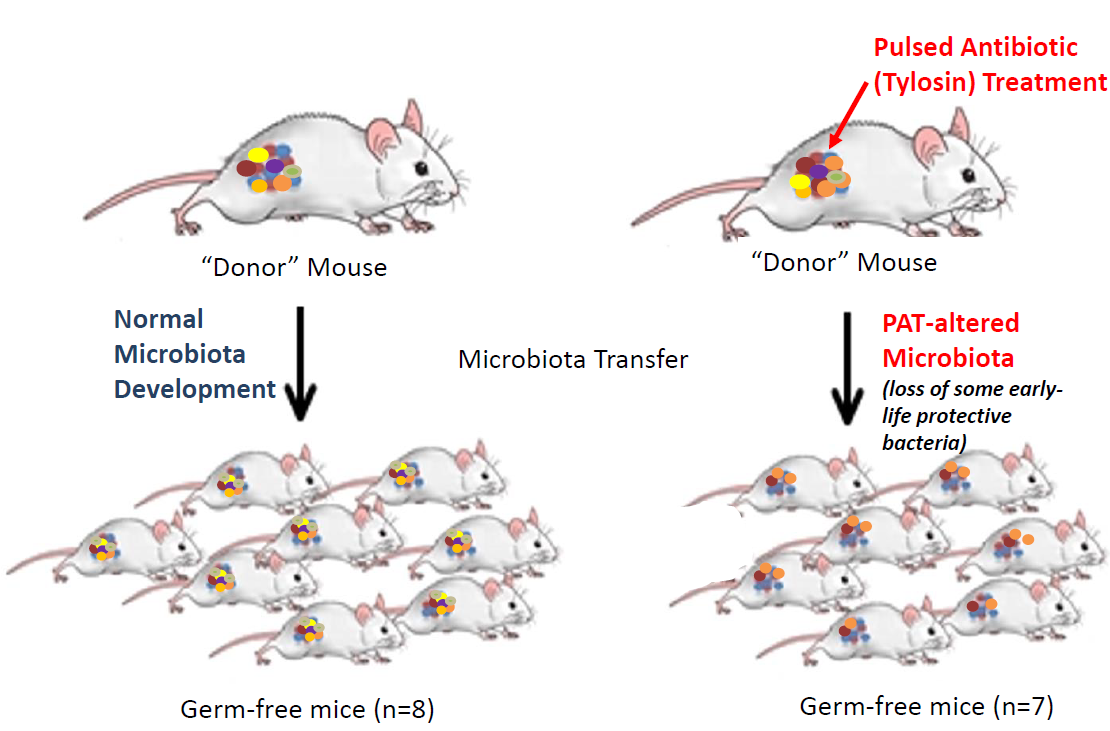
\includegraphics[scale=0.7,height=5.8cm,width=7cm]{rat.PNG}
\end{figure}
\column{0.4\textwidth}
\vspace{0.3in}
\begin{itemize}
\item Measurements:
\begin{enumerate}
\small
\item Microbiome Data
\item Immunological Data
\end{enumerate}
\vspace{0.3in}
\item Research question:
\textcolor{red}{Is the PAT altered Microbiota sufficient to alter Intestinal Immunity?}
\end{itemize}

\end{columns}
\end{frame}


\begin{frame}{\huge{Immunological data}}
\begin{columns}
\column{0.6\textwidth}
\begin{figure}[H]
\centering
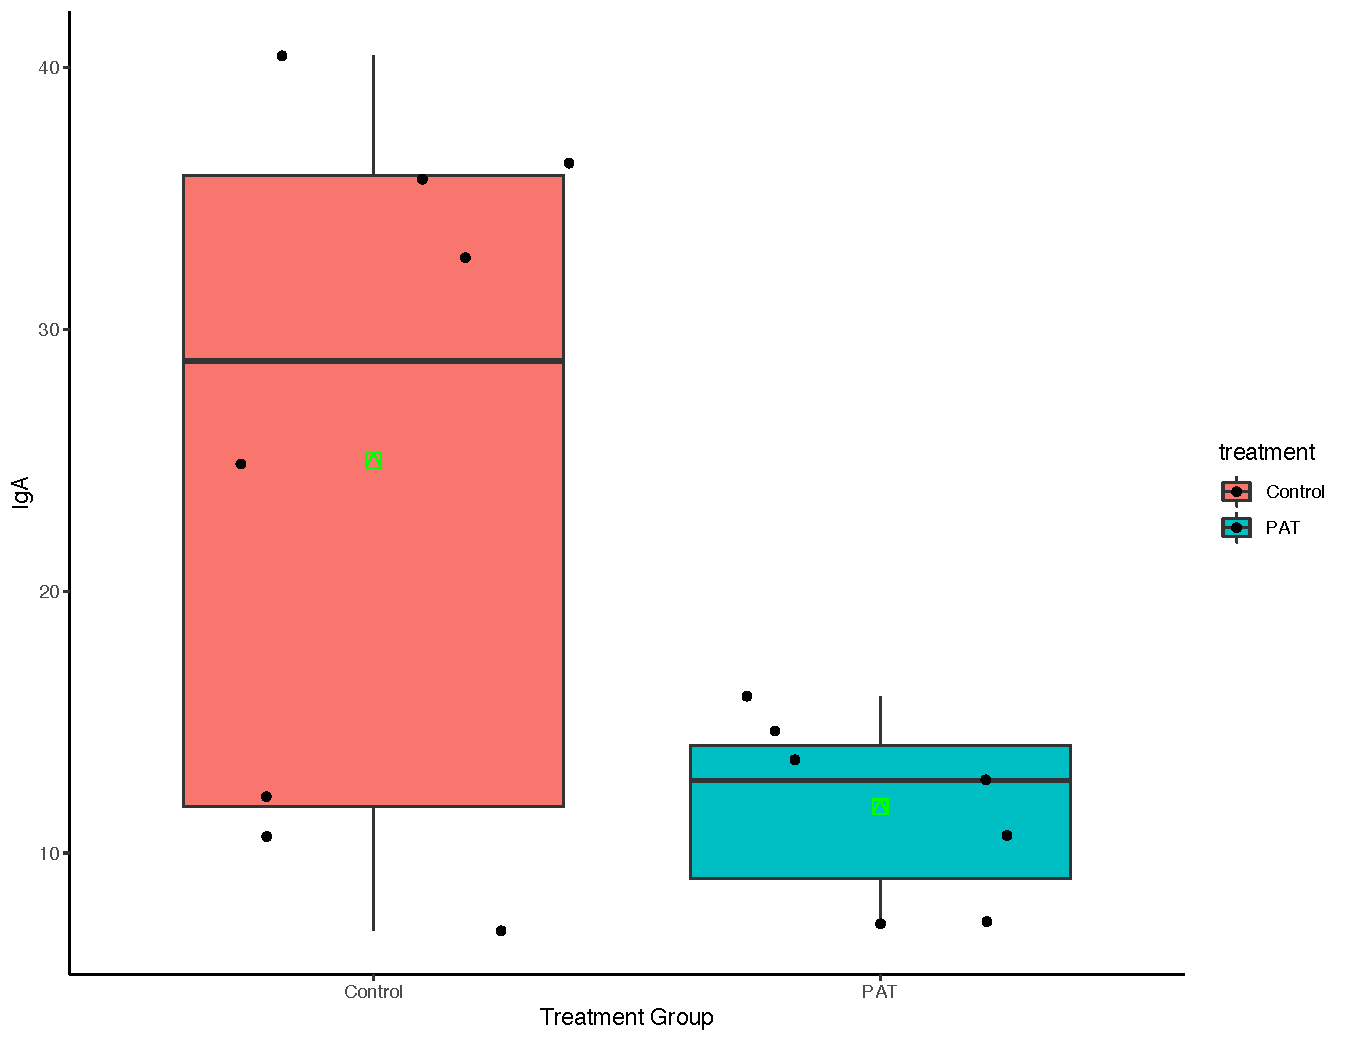
\includegraphics[scale =0.4,height=6.6cm,width=7.5cm]{a.pdf}
\end{figure}

\column{0.4\textwidth}
\begin{itemize}
\small
\item Immunity: Measured by IgA level
\item Analysis: Truncated at Day20
\end{itemize}
\begin{figure}[H]
\centering
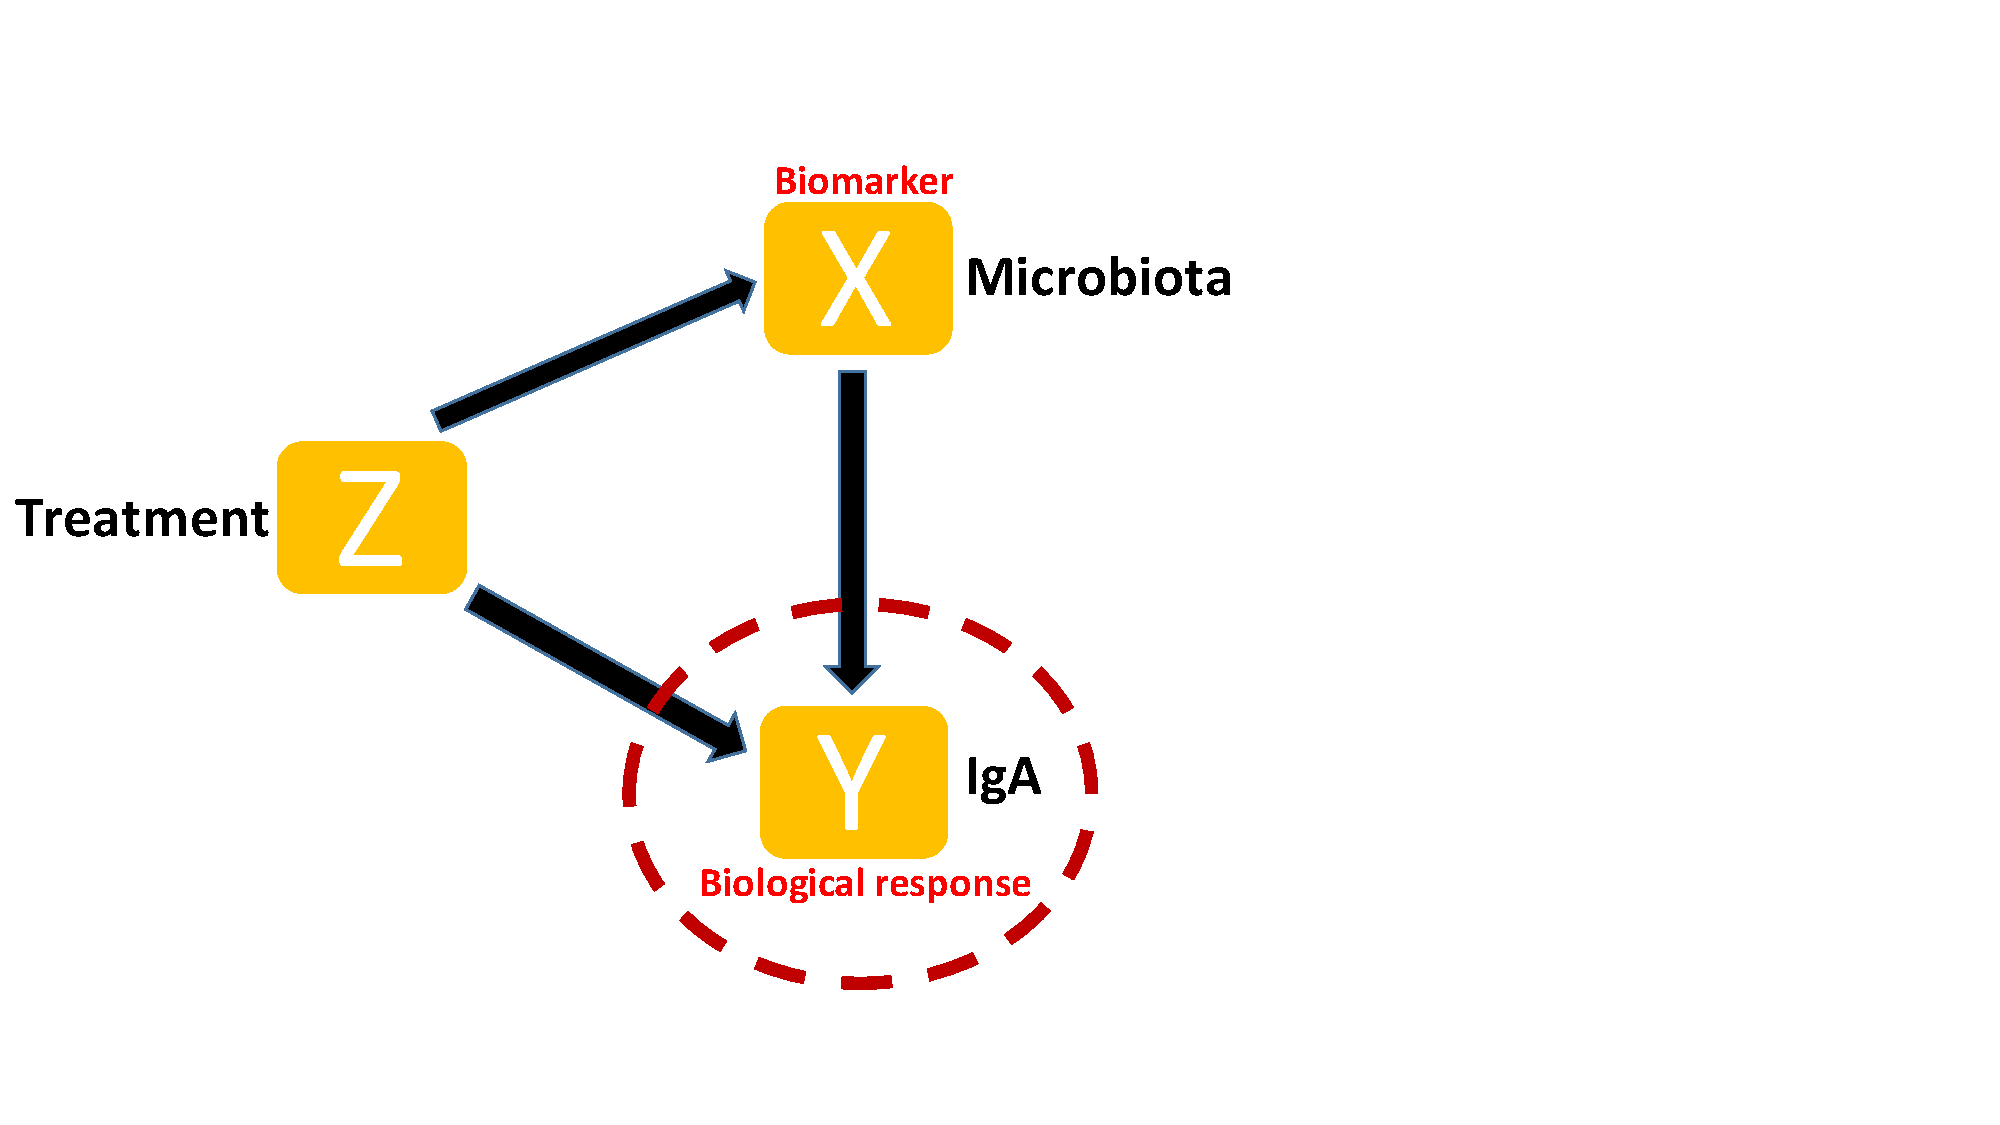
\includegraphics[scale =0.2,height=4cm,width=3.9cm]{ii.pdf}
\end{figure}
\end{columns}
\end{frame}

\begin{frame}{\huge{Microbiome data(1)}}
\begin{figure}[H]
\centering
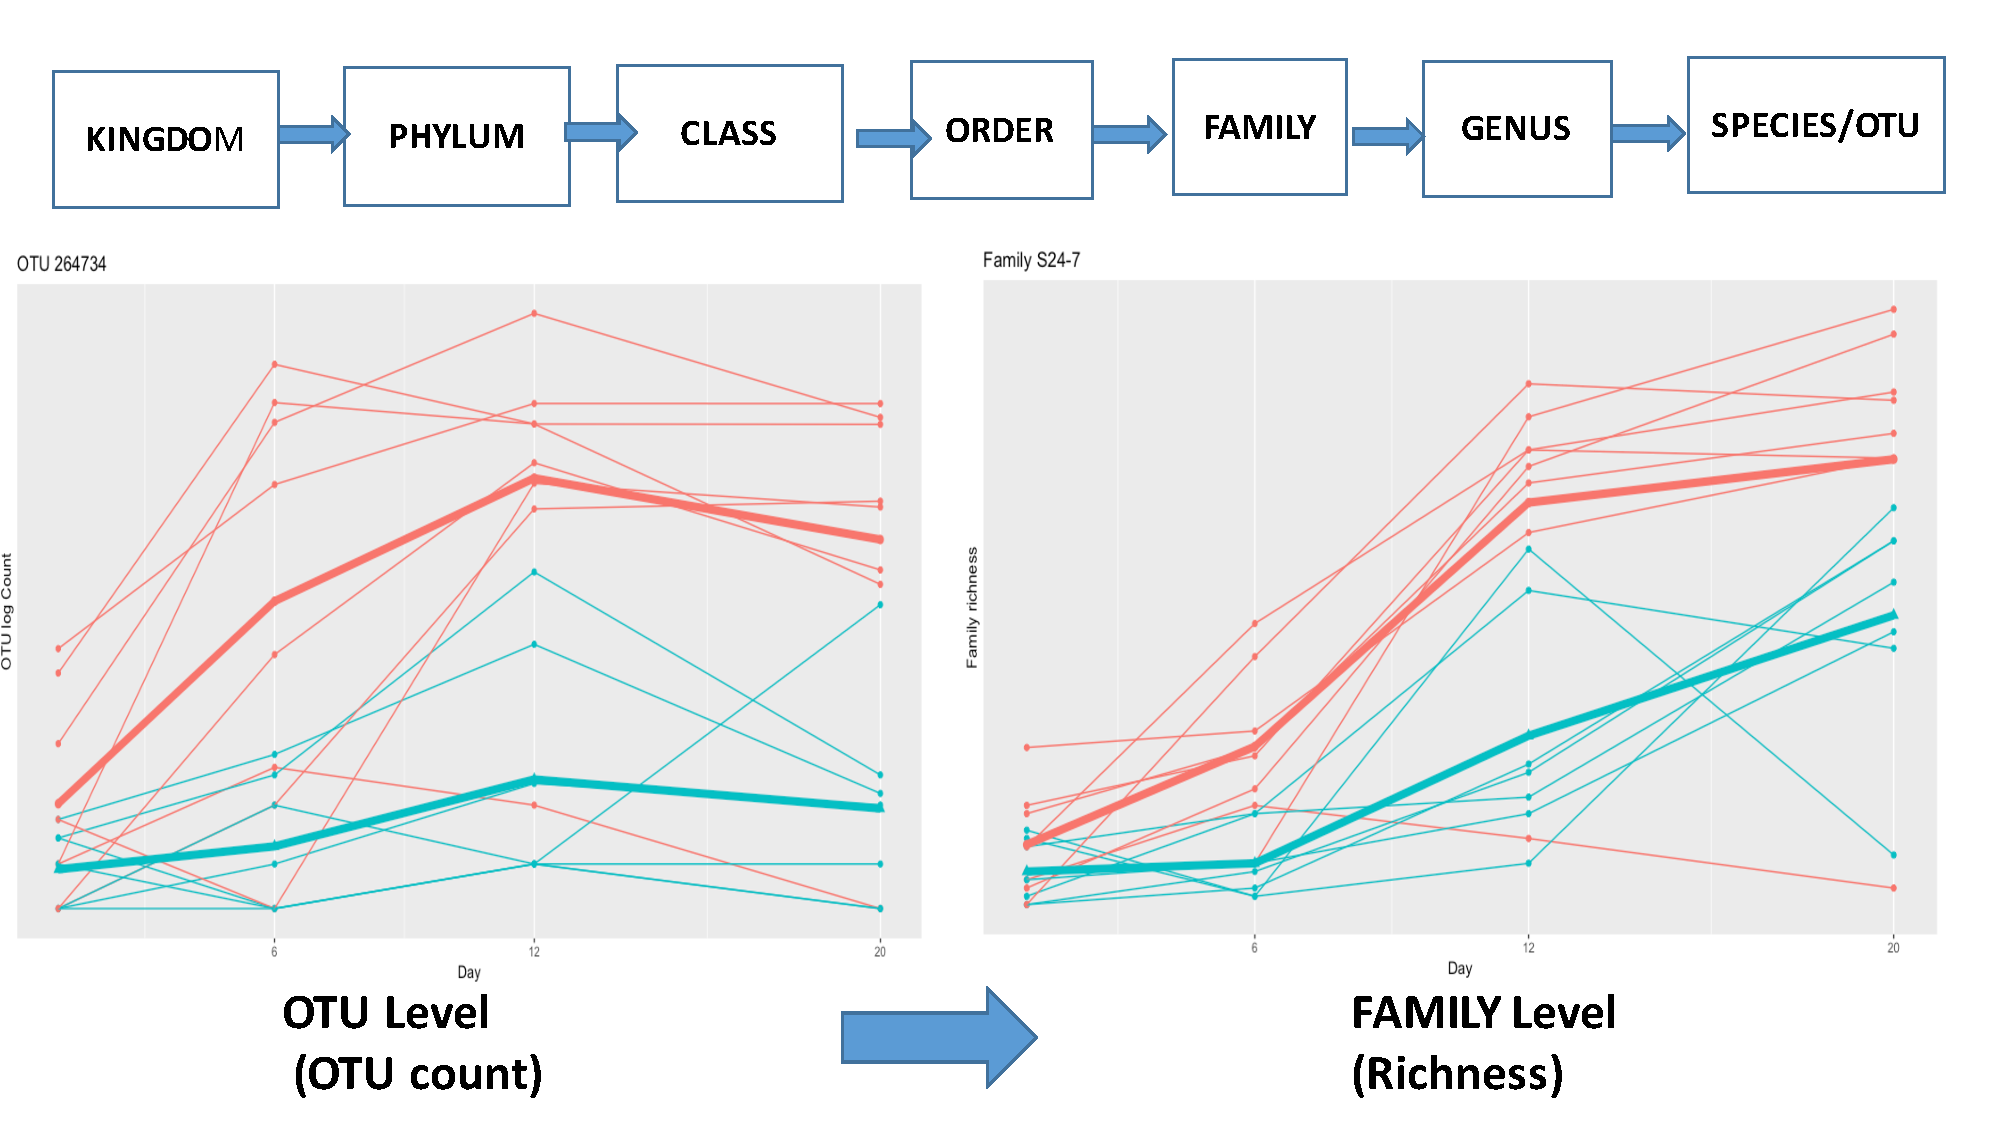
\includegraphics[scale=9,height=6.8cm,width=11.7cm]{otufam.pdf}
\end{figure}
\end{frame}


\begin{frame}{\huge{Microbiome data(2)}}
\begin{columns}
\column{0.6\textwidth}
\begin{figure}[H]
\centering
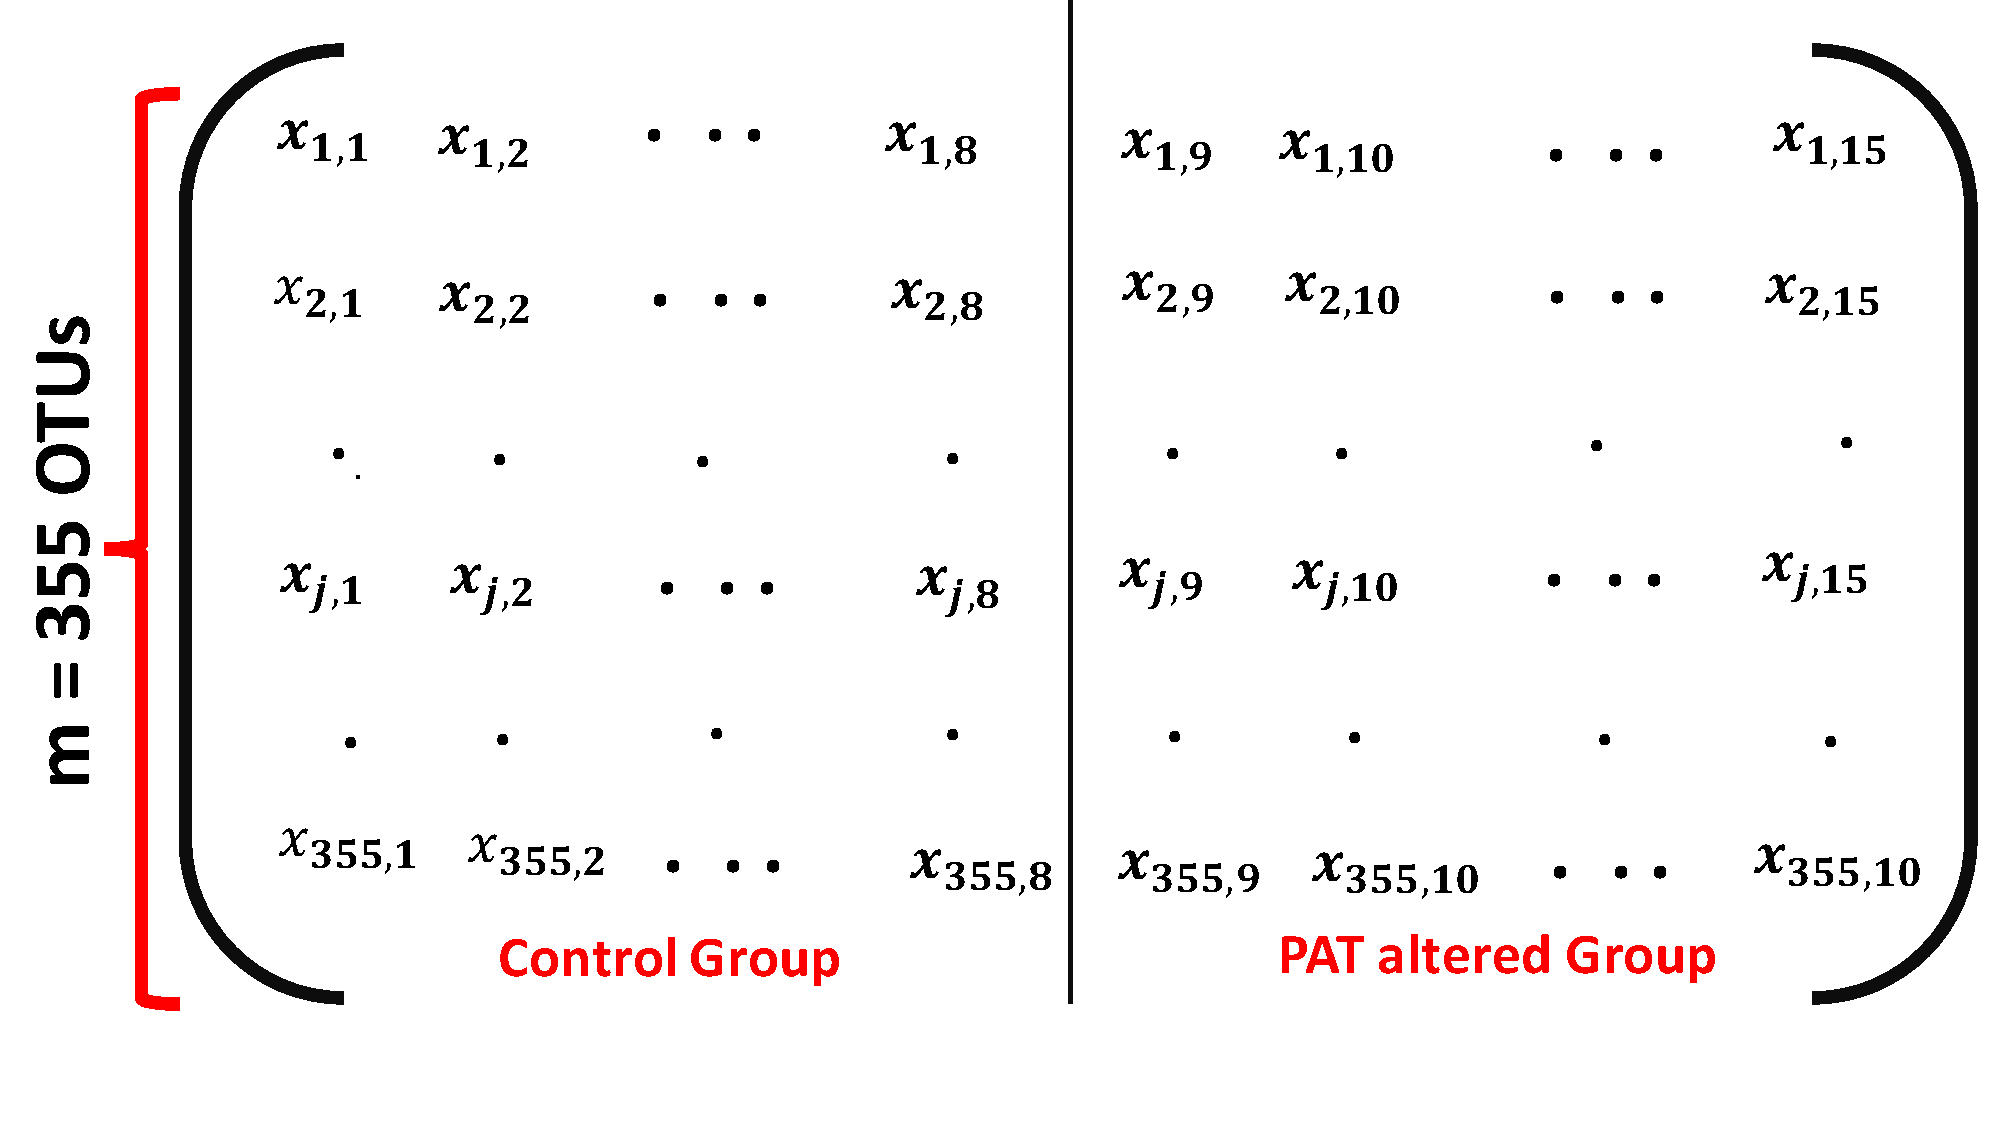
\includegraphics[scale =0.4,height=6.6cm,width=7cm]{ootu.pdf}
\end{figure}

\column{0.4\textwidth}
\begin{itemize}
\small
\item \small{Similar in structure to other omics data: gene expression data, metabolic data...}
\end{itemize}
\begin{figure}[H]
\centering
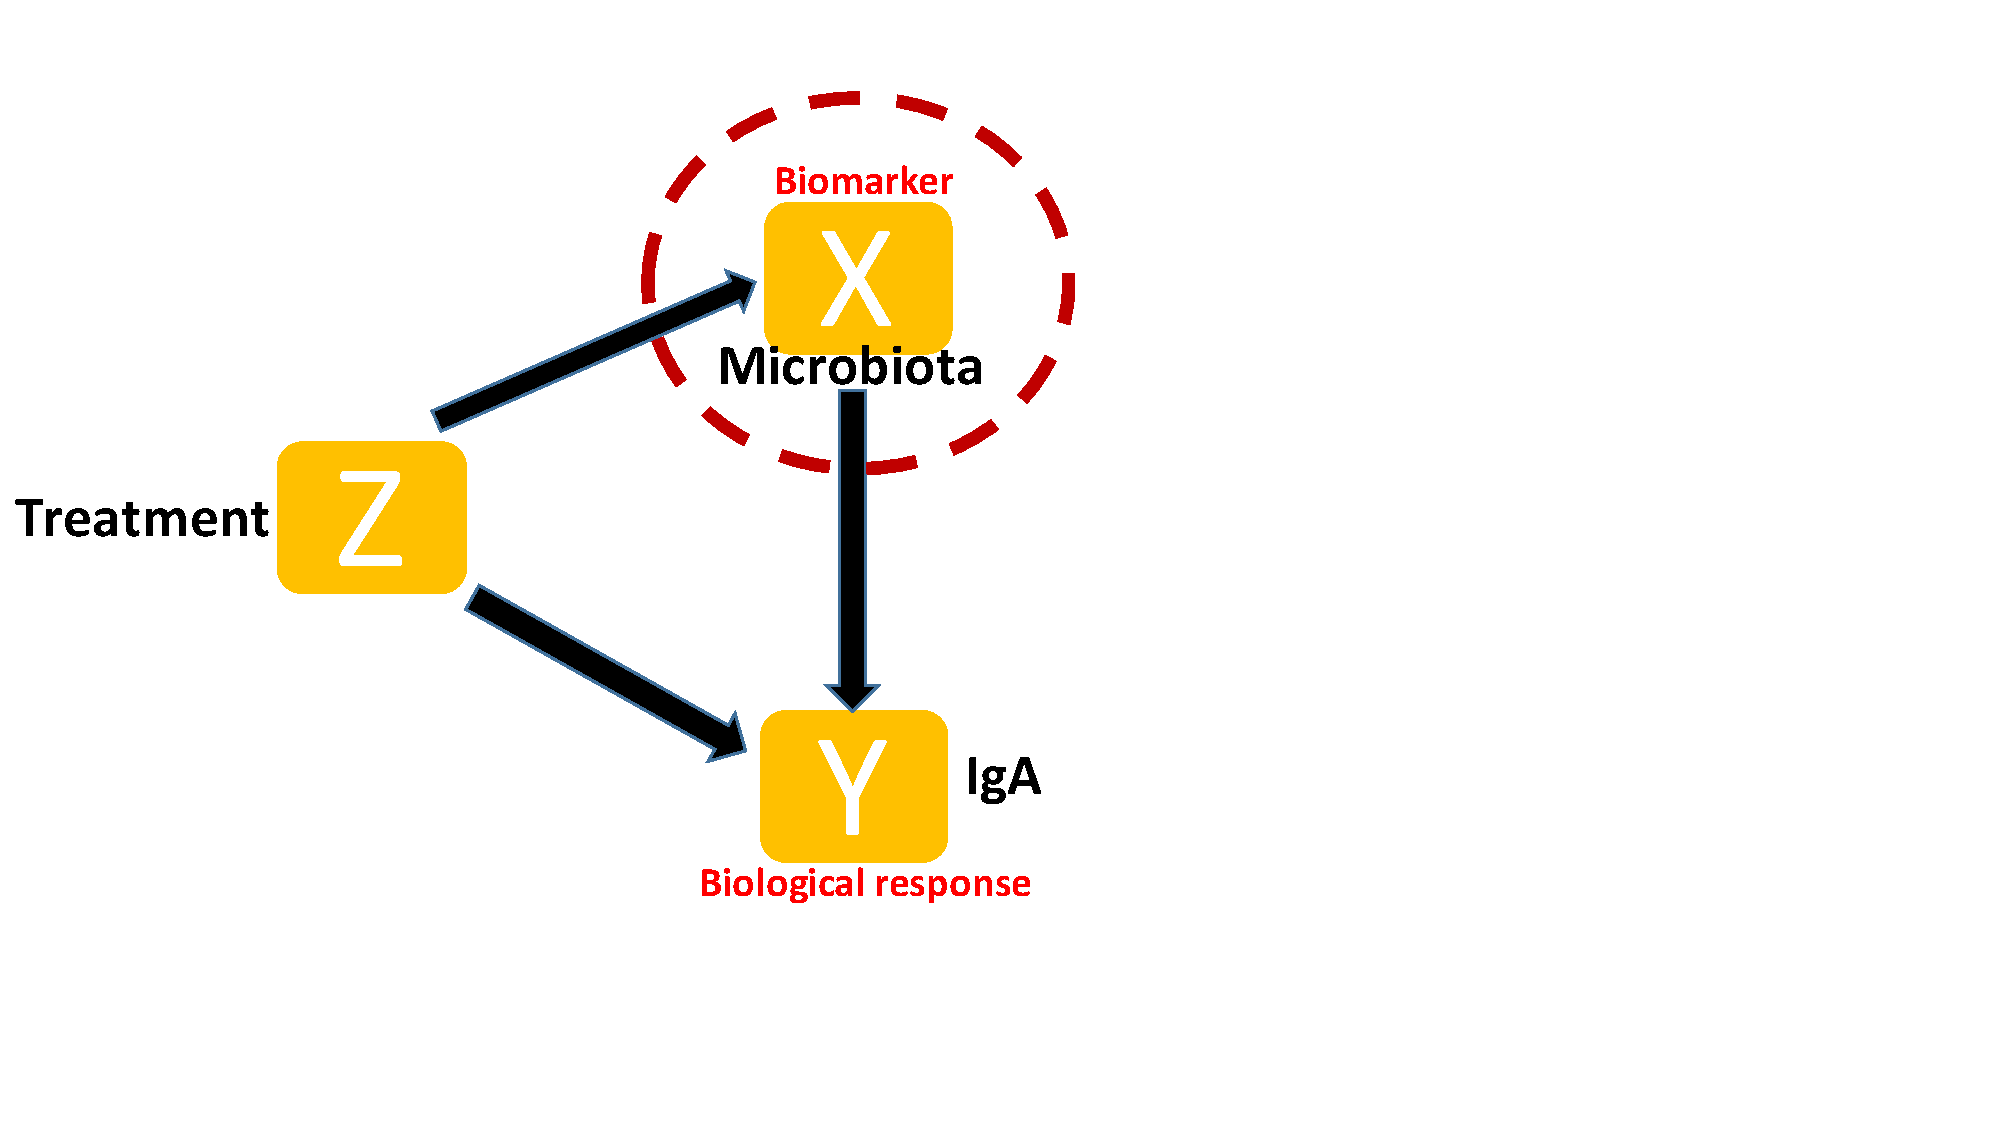
\includegraphics[scale =0.2,height=4cm,width=3.9cm]{mm.pdf}
\end{figure}
\end{columns}
\end{frame}

\begin{frame}{\huge{Data structure}}
\begin{itemize}
\item Repeated measurements  at 4 time points
\item 355 OTU's = 30 families
\item A subject : Mouse
\item Observation unit = $\{
\bm{Z_i,Y_i,X_{ij}}
\}$
%\item 15 germ free mice: 7(PAT) and 8(Control)
$$ Y = \left[ \begin{array}{c}
Y_1\\
Y_2\\
\vdots\\
Y_{15}
\end{array} \right], X = \left[ \begin{array}{cccc}
X_{1,1} & X_{1,2} & \cdots & X_{1,15} \\
X_{2,1} & X_{2,2} & \cdots & X_{2,15} \\
\vdots & \vdots & \vdots & \vdots \\
X_{30,1} & X_{30,2} & \cdots & X_{30,15} \\
\end{array}
\right], Z =  \ \ \left[ \begin{array}{c}
Z_1\\
Z_2\\
\vdots\\
Z_{15}
\end{array}
\right]$$
\item \alert{Richness:} Number of nonzero OTUs for a subject
\item \alert{Family Level richness:}  Richness belonging to a particular family
%\item $Y$ = log(IgA) \alert{(Clinical endpoint)}, $X$ =  family level richness \alert{(Biomarker)}, $Z$ = Treatment \alert{(PAT \& Control)}
\end{itemize}
\end{frame}

\begin{frame}{Family richness over time}
\begin{figure}[H]
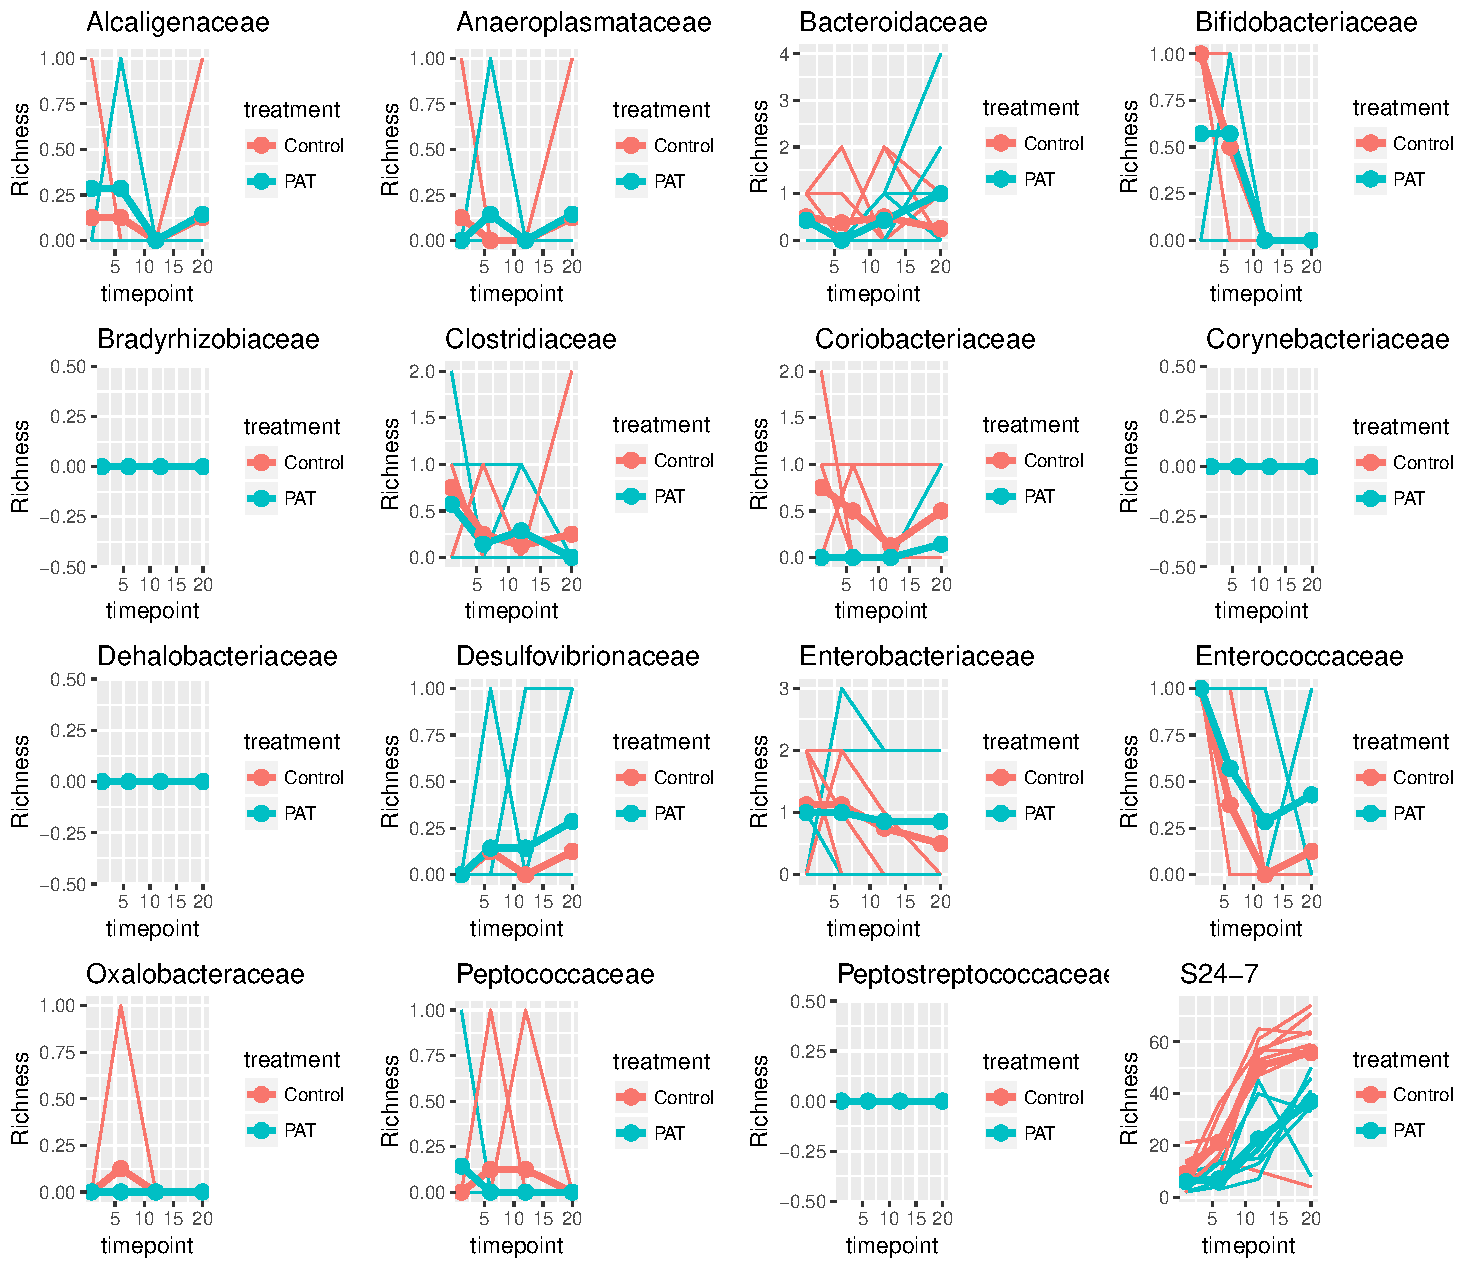
\includegraphics[scale=0.35,height=7cm,width=11.5cm]{newg.pdf}
\end{figure}
\end{frame}

\section{Results}
\subsection{}
\begin{frame}{\huge{Bayesian Variable Selection formulation}}
\small
\begin{figure}[H]
\centering
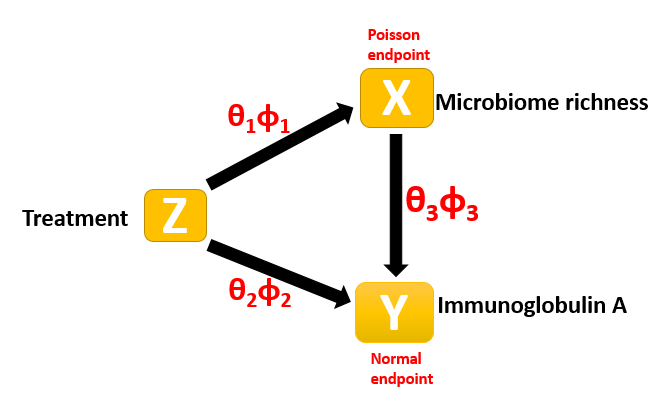
\includegraphics[scale=0.4,height=3.5cm]{hm.PNG}
\end{figure}

\begin{columns}
\column{0.5\textwidth}
$X_i \sim Pois(\lambda_i)$\\
$log(\lambda_i) = \mu_x + \alert{ \phi_1} ^{*}\theta_1 Z_i$ \\
\vspace{0.1in}
$Y_i \sim N(\mu_i,\tau)$\\
$\mu_i = \mu_y + \alert{ \phi_2} ^{*}\theta_2 Z_i + \alert{ \phi_3} ^{*} \theta_3 X_i$ \\ \\

\column{0.5\textwidth}
 $\alpha = \alert{ \phi_1} ^{*}\theta_1; \ \alert{ \phi_1}$=1 \text{then} $\alpha = \theta_1$\\
$\beta = \alert{ \phi_2} ^{*}\theta_2; \ \alert{ \phi_2}$=1 \text{then} $\beta = \theta_2$\\
$\gamma = \alert{ \phi_3} ^{*}\theta_3; \ \alert{ \phi_3}$=1 \text{then} $\gamma = \theta_3$
\end{columns}
\center{\alert{Priors specification}}\\
$\tau \sim Gamma(0.00001, 0.00001) \ \ \ \ \ \ \ \ \ \ \ \ \ \mu_{x}, \mu_{y, }, \alpha , \beta, \gamma \sim N(0, 0.00001)$\\

$\alert{ \phi_i} \sim B(\pi_i) \ \ \ \text{and} \ \ \ \ \ \pi_i \sim U(0,1)$\\

\end{frame}


% \begin{frame}{Models configuration}
% \small
% \vspace{0.5cm}
% \begin{itemize}
% \item The configuration of $\alert{ \phi}$ define uniquely the 8 models
% \end{itemize}
% \vspace{0.3cm}
% For example:
% \vspace{0.2cm}

% \begin{minipage}[t]{0.48\linewidth}
% \begin{figure}[H]
% \caption{Model 6}
% \includegraphics[scale=0.4]{eg1.PNG}
% \end{figure}
% \center{$\alert{ \phi} = \{\alert{ 1}, \alert{ 1}, \alert{ 0}\}$}
% $$\begin{array}{l}
%  \begin{pmatrix} 
% \text{log}(\lambda_i) \\
% \mu_i 
% \end{pmatrix}=  
%       \begin{pmatrix} 
% \mu_X + \alpha Z_i\\ \\
% \mu_Y + \beta Z_i
% \end{pmatrix}
% \end{array}$$
% \end{minipage}
% \begin{minipage}[t]{0.48\linewidth}
% \begin{figure}[H]
% \caption{Model 5}
% \includegraphics[scale=0.4]{eg2.PNG}
% \end{figure}
% \center{$\alert{ \phi} = \{\alert{ 1}, \alert{ 0}, \alert{ 1}\}$}
% $$\begin{array}{l}
%  \begin{pmatrix} 
% \text{log}(\lambda_i) \\
% \mu_i 
% \end{pmatrix}=  
%       \begin{pmatrix} 
% \mu_X + \alpha Z_i\\ \\
% \mu_Y + \gamma X_i
% \end{pmatrix}
% \end{array}$$
% \end{minipage}

% \end{frame}



%%%%%%%%%%%%%%%%%%%%%%%%%%%%%%%%%%%%%%%%%%%%%%
\begin{frame}{\huge{Design matrix for the indicators}}
%\vspace{0.1cm}
\medium
\begin{itemize}
\item Matrix of indicator for  the 8 models:
\end{itemize}
\centering{
$\Phi$ = \(
   \begin{Bmatrix} 
   \alert{\phi_1}&\alert{\phi_2}&\alert{\phi_3}\\
   \hline
      0 & 0 & 0\\ 
      1 & 0 & 0 \\ 
      0 & 1 & 0 \\
      0 & 0 & 1 \\
      1 & 0 & 1\\
      1&1&0\\
      0&1&1\\
      1&1&1
   \end{Bmatrix}
\) \\}
 %Let Q = 
\vspace{0.5cm}
\begin{itemize}
\item Unique identification of a model
\end{itemize}
C = \{1, 2, 4\} \\ 
$T_r = 1 + \Phi C^T$
\end{frame}

\begin{frame}{\huge{Models' posterior  probability}}
\begin{itemize}
\item Transformation rule for each model\\
$$T_r =
    \begin{cases}
       1,  \alert{\textbf{.}} & \text{for} \ \ \ \alert{\phi} = (\alert{\phi_1} = 0, \ \ \ \alert{\phi_2} = 0, \ \ \ \ \alert{\phi_3} = 0), \ \ \ \ \text{model} \ m_1\\
      2, & \text{for} \ \ \ \alert{\phi} = (\alert{\phi_1} = 1, \ \ \ \alert{\phi_2} = 0, \ \ \ \ \alert{\phi_3} = 0), \ \ \ \ \text{model} \ m_2\\
      3, & \text{for} \ \ \ \alert{\phi} = (\alert{\phi_1} = 0, \ \ \ \alert{\phi_2} = 1, \ \ \ \ \alert{\phi_3} = 0), \ \ \ \ \text{model} \ m_3\\
      5, & \text{for} \ \ \ \alert{\phi} = (\alert{\phi_1} = 0, \ \ \ \alert{\phi_2} = 0, \ \ \ \ \alert{\phi_3} = 1), \ \ \ \ \text{model} \ m_4\\
      6, & \text{for} \ \ \ \alert{\phi} = (\alert{\phi_1} = 1, \ \ \ \alert{\phi_2} = 0, \ \ \ \ \alert{\phi_3} = 1), \ \ \ \ \text{model} \ m_5\\
      4, & \text{for} \ \ \ \alert{\phi} = (\alert{\phi_1} = 1, \ \ \ \alert{\phi_2} = 1, \ \ \ \ \alert{\phi_3} = 0), \ \ \ \ \text{model} \ m_6\\
      7, & \text{for} \ \ \ \alert{\phi} = (\alert{\phi_1} = 0, \ \ \ \alert{\phi_2} = 1, \ \ \ \ \alert{\phi_3} = 1), \ \ \ \ \text{model} \ m_7\\
      8, & \text{for} \ \ \ \alert{\phi} = (\alert{\phi_1} = 1, \ \ \ \alert{\phi_2} = 1, \ \ \ \ \alert{\phi_3} = 1), \ \ \ \ \text{model} \ m_8
\end{cases}$$
\vspace{0.15in}
\item Posterior probability of transformation
    $$p(m_4|\alert{\phi}, \text{data}) = p(T_r = 5|\alert{\phi}, \text{data})$$
    \end{itemize}
\end{frame}

%%%%%%%%%%%%%%%%%%%%%%%%%%%%%%%%%%%%%%%%%%%%%%
\begin{frame}{\huge{Inclusion probability (per day)}}
\begin{figure}[H]
\begin{minipage}{0.5\textwidth}
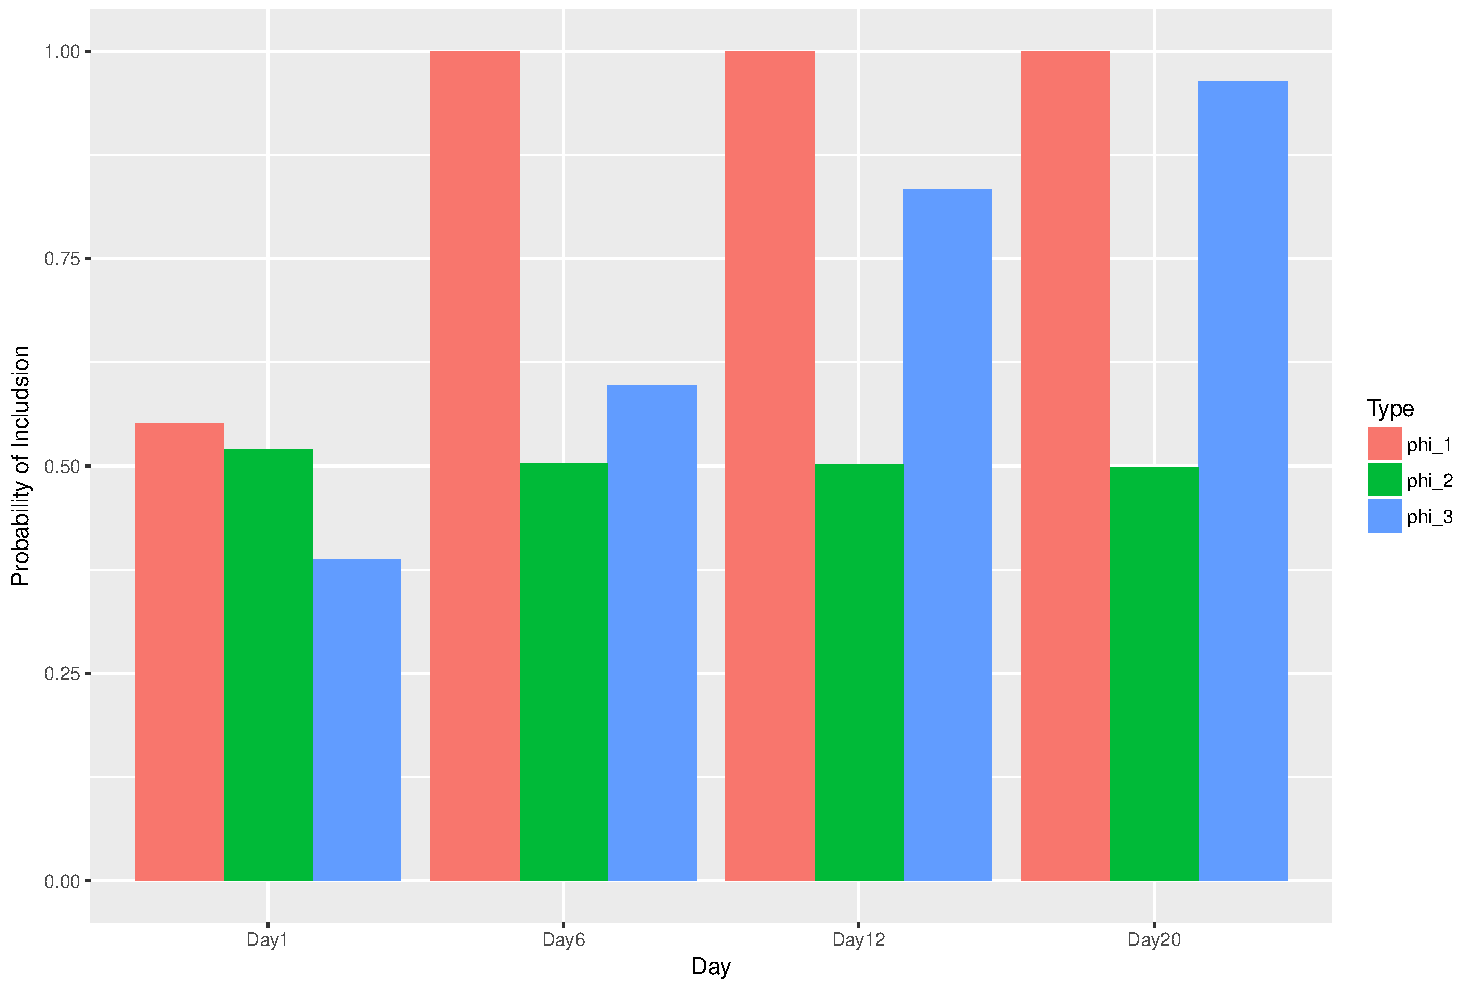
\includegraphics[scale=0.3,height=7cm,width=7cm]{ind.pdf}
\end{minipage}
\hfill
\begin{minipage}{0.3\textwidth}
\centering
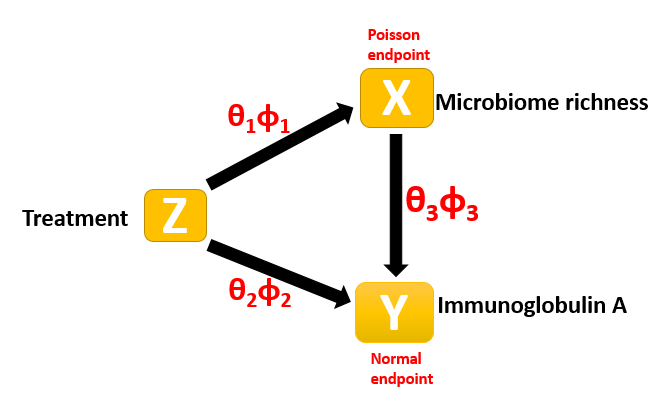
\includegraphics[scale=0.3]{hm.PNG}
\begin{itemize}
\small
\item $P(\phi_3=1|data$) develops over time
\end{itemize}
\end{minipage}
\end{figure}
\end{frame}


% \begin{frame}{\huge{Models' posterior probability (per day)}}
% \begin{figure}[H]
% \begin{minipage}{0.5\textwidth}
% 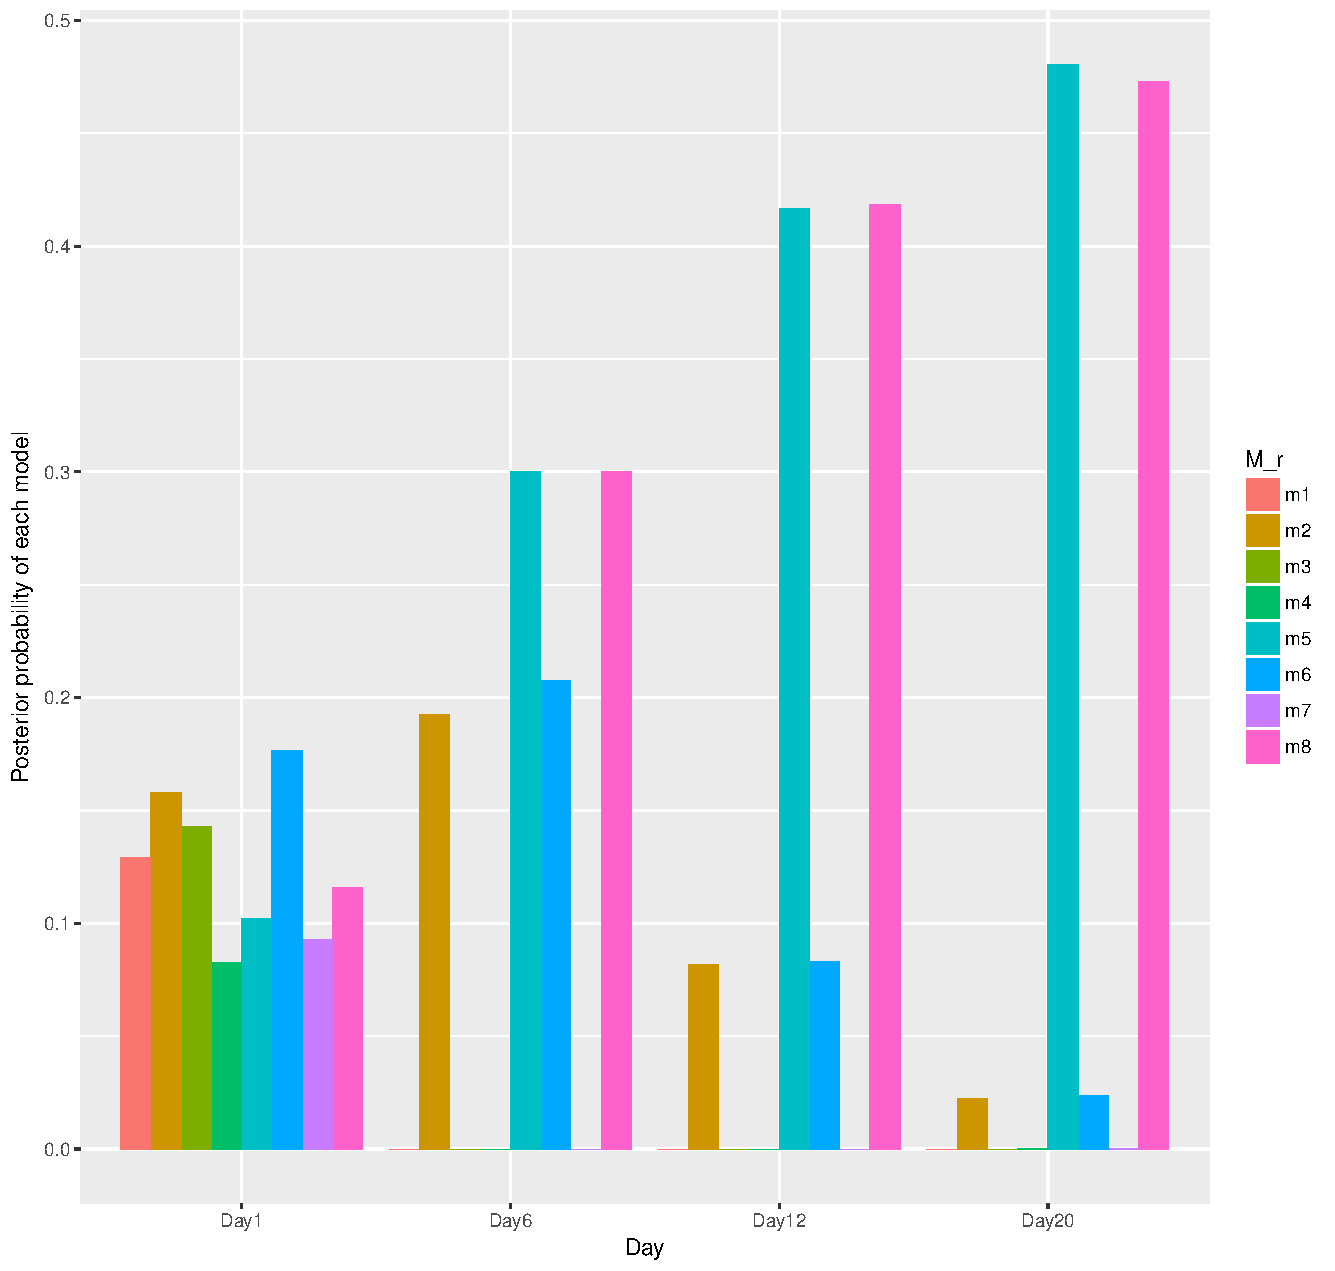
\includegraphics[scale=0.5,height=7cm,width=7cm]{Rplot02.pdf}
% \end{minipage}
% \hfill
% \begin{minipage}{0.3\textwidth}
% %\vspace{1.2cm}
% 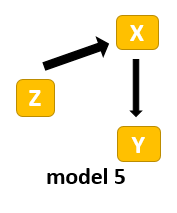
\includegraphics[scale=0.5]{m5.PNG}\\

% %\vspace{0.5cm}
% 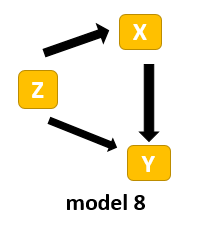
\includegraphics[scale=0.4]{m8.PNG}

% \end{minipage}
% \end{figure}
% \end{frame}

%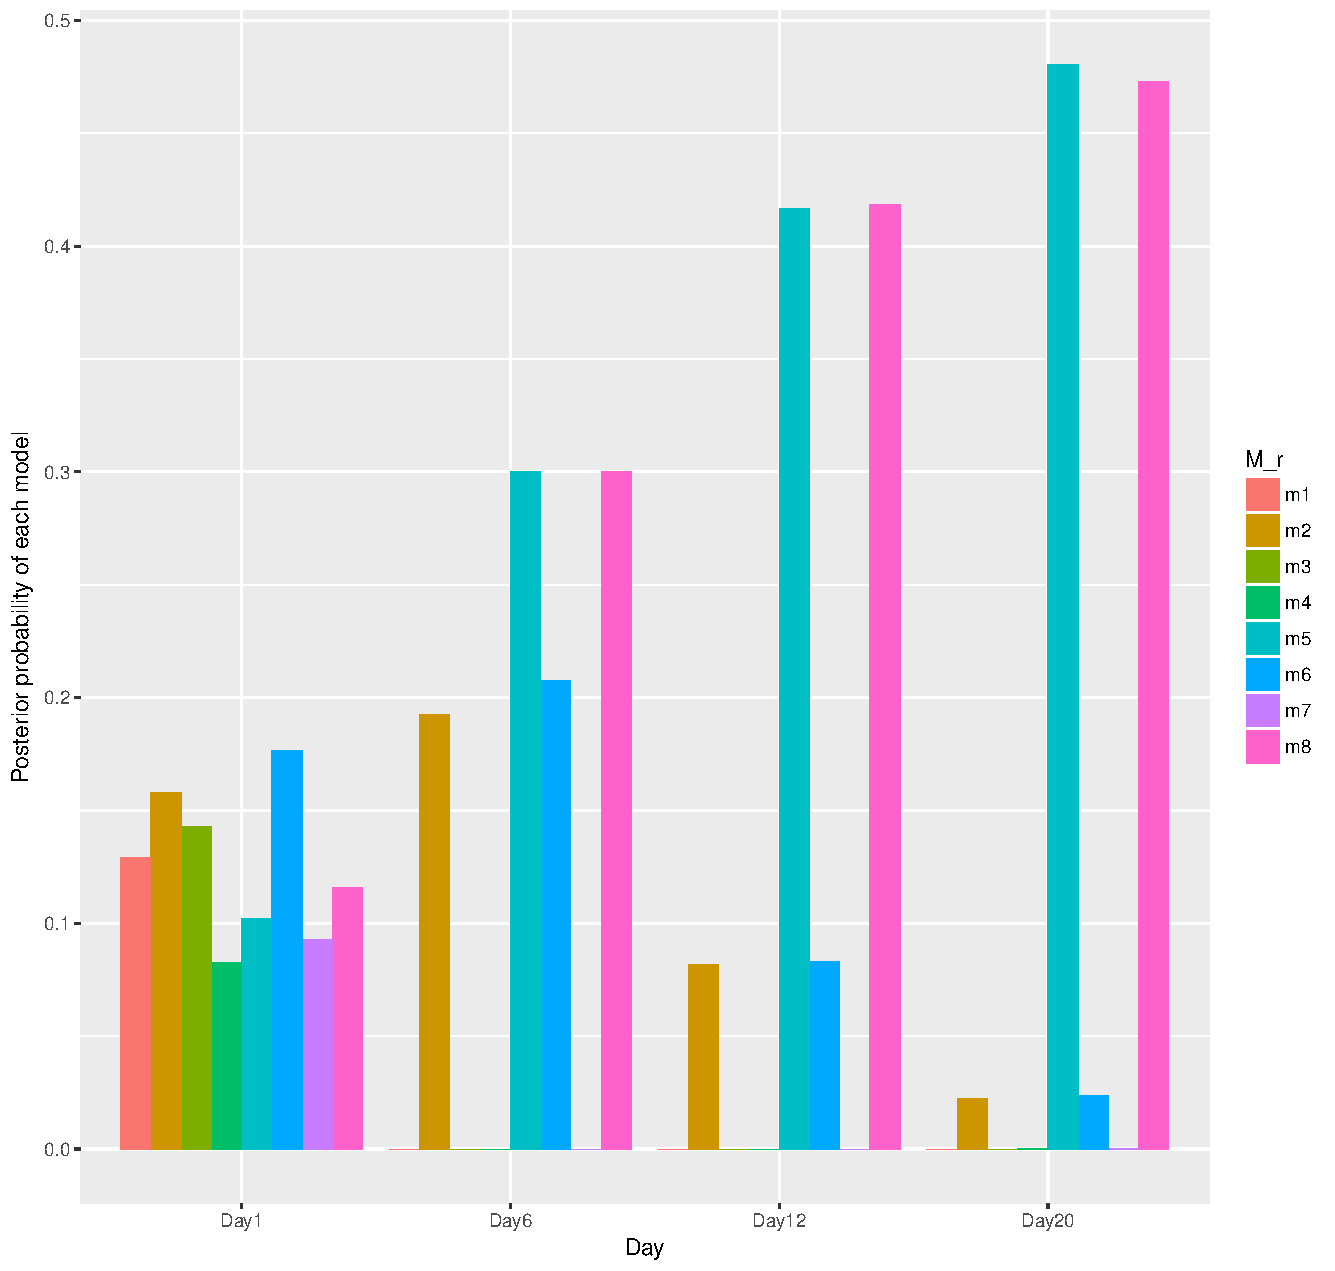
\includegraphics[scale=0.3,height=6cm,width=9cm]{Rplot02.pdf}
%[scale=0.5,height=6cm,width=1cm]{m6.PNG}

\begin{frame}{\huge{What is the probability for X to be a biomarker at day 20?}}

\begin{figure}[H]
\centering
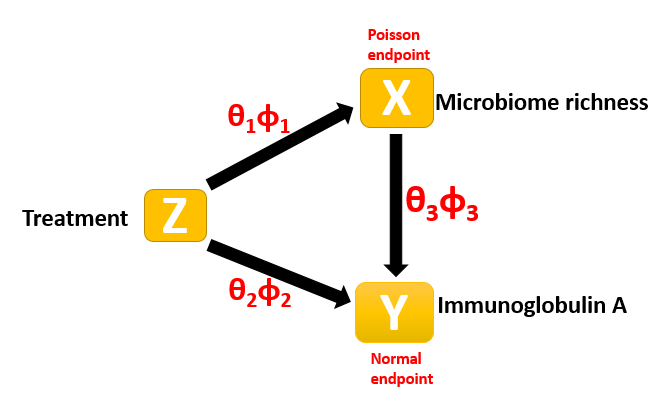
\includegraphics[scale=0.6]{hm.PNG}
\end{figure}
\small
$P(\phi_1 = 1|data) = P(m_2) + P(m_5) + P(m_6) + P(m_8) = 0.9996$\\
$P(\phi_2 = 1|data) = P(m_3) + P(m_6) + P(m_7) + P(m_8) = 0.5007$\\
\center{\underline{Probability that X is a biomarker}}\\
$\alert{P(\phi_3 = 1|data) = P(m_4) + P(m_5) + P(m_7) + P(m_8) = 0.96045}$
\end{frame}

\section{Conclusion and further research}
\subsection{}
\begin{frame}{\huge{Conclusion and Further Research}}
\vspace{-0.2in}
\begin{block}{\huge{Conclusion}}
\end{block}
\begin{itemize}
\item Bayesian extension of the JM for all type of distribution
\item The probability of inclusion as a measure of surrogacy
\item Richness as a biomarker was seen to be \alert{highly related to the IgA over time} 
\end{itemize}

\begin{block}{\huge{Further research}}
\end{block}
\begin{itemize}
\item To take into account the \alert{longitudinal information}
\item Incorporate other features
\item Testing the method on \alert{a better dataset (small sample and few active features)}
\item  Establish a \alert{connection between our method and the information criteria approach through simulation.}
\end{itemize}

\end{frame}


\end{document}
